\documentclass[portrait,a0,final,20pt]{a0poster}
%%%Load packages
\usepackage{multicol} 			%2-column layout
% \setlength\columnsep{8pt} % This is the default columnsep for all pages
\usepackage[left=2cm,right=2cm,bottom=2cm,top=0cm]{geometry}			%Reset margins
\usepackage{helvet}				%Load Helvetica font & CM math
\usepackage{color}				%Needed for colour boxes & coloured text
% \usepackage{graphics}
\usepackage{graphicx}
\usepackage{subcaption}
\usepackage[font=Large,labelfont=bf]{caption}
\usepackage{float}
\usepackage{tikz}
\usetikzlibrary{arrows,positioning, shapes.symbols,shapes.callouts,patterns,shapes,chains,calc,backgrounds,fadings}

\usepackage{titlesec}
\usepackage{tabularx, booktabs} % make width of table columns evenly distributed (see http://tex.stackexchange.com/questions/60601/evenly-distributing-column-widths)

\usepackage{enumitem}
\usepackage{animate}[2017/05/18]

\usepackage{hyperref}
\usepackage{xcolor}
\usepackage{newtxtext,newtxmath}

% \usepackage{titlepic}
% \usepackage{columns}

\titlespacing\section{0pt}{10pt plus 4pt minus 2pt}{5pt plus 2pt minus 2pt}
\titlespacing\subsection{0pt}{12pt plus 4pt minus 2pt}{0pt plus 2pt minus 2pt}

\titleformat*{\section}{\Huge\bfseries}
\titleformat*{\subsection}{\Large\bfseries}
\titleformat*{\subsubsection}{\large\bfseries}
\titleformat*{\paragraph}{\large\bfseries}
\titleformat*{\subparagraph}{\large\bfseries}

%%%Define colours and lengths
\definecolor{headingcol}{rgb}{0,0,0}			%Colour of main title
\definecolor{boxcol}{rgb}{0.7,0.2,0.2}		%Edge-colour of box and top banner
\fboxsep=1cm							%Padding between box and text
\setlength{\columnsep}{2cm}				%Set spacing between columns
\renewcommand{\familydefault}{\sfdefault}	%Set main text to sans-serif

%%%Format title
\makeatletter							%Needed to include code in main file
\renewcommand\@maketitle{%
\null									%Sets position marker
% \vspace{5em}
{
\color{headingcol}\sffamily\VeryHuge		%Set title font and colour
\@title \par}%
\vskip 0.6em%
{
\color{black}\sffamily\LARGE				%Set author font and colour
\lineskip .5em%
\begin{tabular}[t]{l}%
\@author
\end{tabular}\par}%
\vskip 1cm
\par
}
\makeatother



\title{Disease Knowledge Transfer across Neurodegenerative Diseases}

\newcommand{\inst}[1]{$^{#1}$}

% \author{\Large{R\u{a}zvan V. Marinescu\inst{1}, Neil P. Oxtoby\inst{1}, Alexandra L. Young\inst{1}, Arman Eshaghi\inst{2}, Peter A. Wijeratne\inst{1}, Daniel C. Alexander\inst{1}}\\
% \begin{tabular}{l p{1cm} l p{1cm} l}
% \large{$^1$Centre for Medical Image Computing, University College London}  & & \large{$^2$Queen Square MS Centre, UCL Institute of Neurology} \\
% \end{tabular}
% }

\author{R\u{a}zvan V. Marinescu\inst{1,2}, Marco Lorenzi\inst{5}, Stefano B. Blumberg\inst{1}, Alexandra L. Young\inst{1}, Pere Planell-Morell\inst{1}, Neil P. Oxtoby\inst{1}, Arman Eshaghi\inst{1,3}, Keir X. Young\inst{4}, Sebastian J. Crutch\inst{4}, Polina Golland\inst{2}, Daniel C. Alexander\inst{1}\\
\begin{tabular}{l p{1cm} l p{1cm} l}
\large{$^1$Centre for Medical Image Computing, University College London}  & & \large{$^2$Queen Square MS Centre, UCL Institute of Neurology} \\
\end{tabular}
} 

\newcommand{\fnt}[1]{\LARGE{#1}}



\begin{document}
% \hspace{-3cm}								%Align with edge of page, not margin
% \vspace{2cm}
% \includegraphics[scale=1,trim=0 0 0 200, clip]{Black_Landscape.pdf}

%\colorbox{boxcol}{							%Coloured banner across top
\begin{minipage}{50cm}					%Minipage for title contents
% \vspace{-18cm}
\maketitle
\end{minipage}
%}
% \vspace{-4cm}

\fnt{

\begin{multicols}{2}							
\raggedcolumns							%Don't stretch contents vertically

\pagenumbering{gobble}

%%%Column1
\vspace{-3em}


\section*{Aim}

Propose mechanism to infer progression of non-MRI biomarkers in rare neurodegenerative diseases by leveraging larger datasets of common neurodegenerative diseases.

\section*{Why}


\newcommand{\lp}{\lambda_{d_i}^{\psi(k)}}
\newcommand{\lpuu}{\lambda_{d_i}^{\psi(k),(u)}}
\newcommand{\lpum}{\lambda_{d_i}^{\psi(k),(u-1)}}

\begin{itemize}
 \item Datasets on rare neurodegenerative diseases (e.g., Posterior Cortical Atrophy) are unimodal (MRI only), cross-sectional and small.
 \item The continuous progression of non-MRI markers in rare neurodegenerative diseases is not well understood
\end{itemize}

% \vspace{-0.5em}


 
% \begin{itemize}
%  \item by transferring knowledge from larger multimodal datasets of typical Alzheimer's disease
%  \item jointly model multiple diseases and multiple modalities
% \end{itemize}




\section*{Method}



% \begin{itemize}
%  \item We propose a joint-disease model called Disease Knowledge Transfer:
 \vspace{1em}
 \begin{figure}[H]
 \centering
  \begin{subfigure}{0.49\columnwidth}
   \centering
   \fnt{1. Each disease characterised by region-specific dysfunction profile}\\
   $ \gamma_{ij}^l = f(\beta_{i} + m_{ij}; \lambda_{d_i}^l) $\\
%    \vspace{0.9em}
   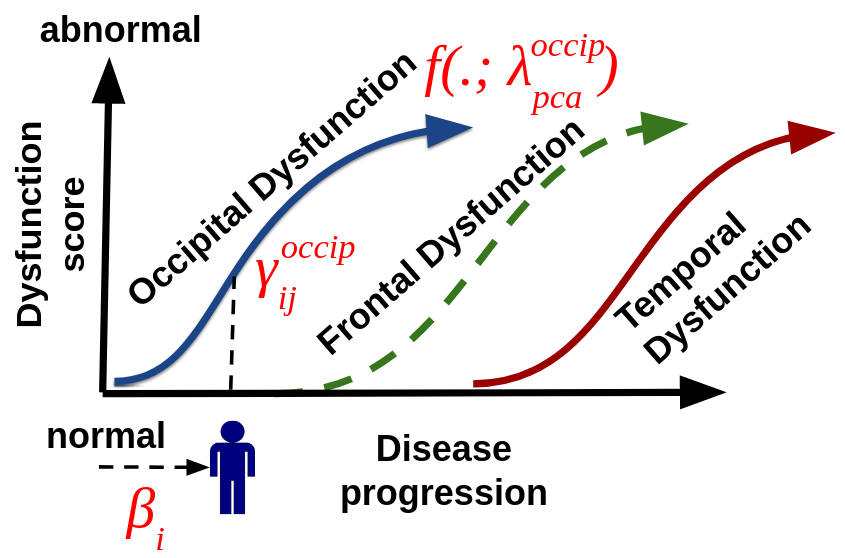
\includegraphics[width=\textwidth]{diseaseEvol}
   
  \end{subfigure}
  \begin{subfigure}{0.49\columnwidth}
   \centering
%    \vspace{-1.2em}
   \fnt{2. Dysfunction score modelled using region-specific biomarkers}\\
   $ p(y_{ijk}|\theta_k, \lp, \beta_{i}, \epsilon_k) = N(y_{ijk}| g( \gamma_{ij}^{\psi(k)} ; \theta_k), \epsilon_k) $
%    \vspace{0.6em}
   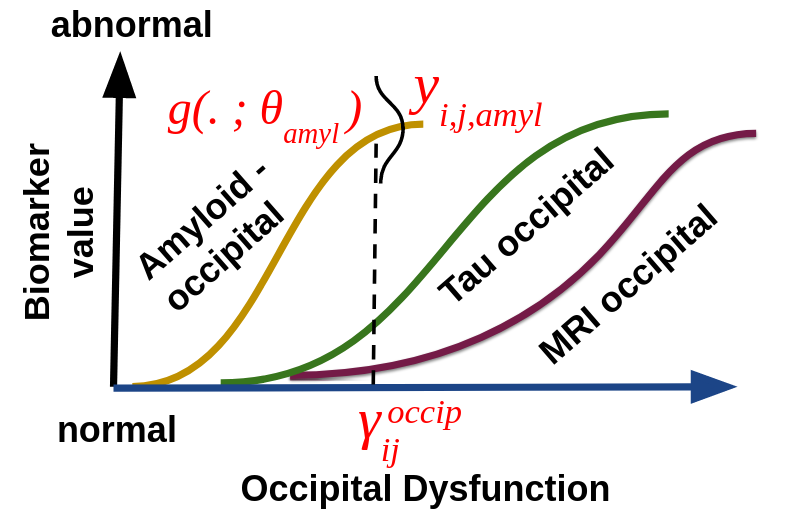
\includegraphics[width=\textwidth]{dysfuncEvol}
  \end{subfigure}

 \end{figure}

 
%    \item each disease has a unique evolution of region-specific dysfunction scores
%    \item each dysfunction score modelled as the unique evolution of biomarkers within that region
 
% \end{itemize}



% \subsection{Method Overview}





% $ p(y_{ijk}|\theta_k, \lp, \beta_{i}, \epsilon_k) = N(y_{ijk}| g( \gamma_{ij}^{\psi(k)} ; \theta_k), \epsilon_k) $





\begin{figure}[H]
 \centering
  \fnt{3. Extend to multiple subjects, biomarkers and diseases}\\
 $ p(\boldsymbol{y}|\theta, \lambda, \beta , \epsilon) = \prod_{(i,j,k) \in \Omega} p(y_{ijk}|\theta_k, \lp, \beta_{i}) $
 
 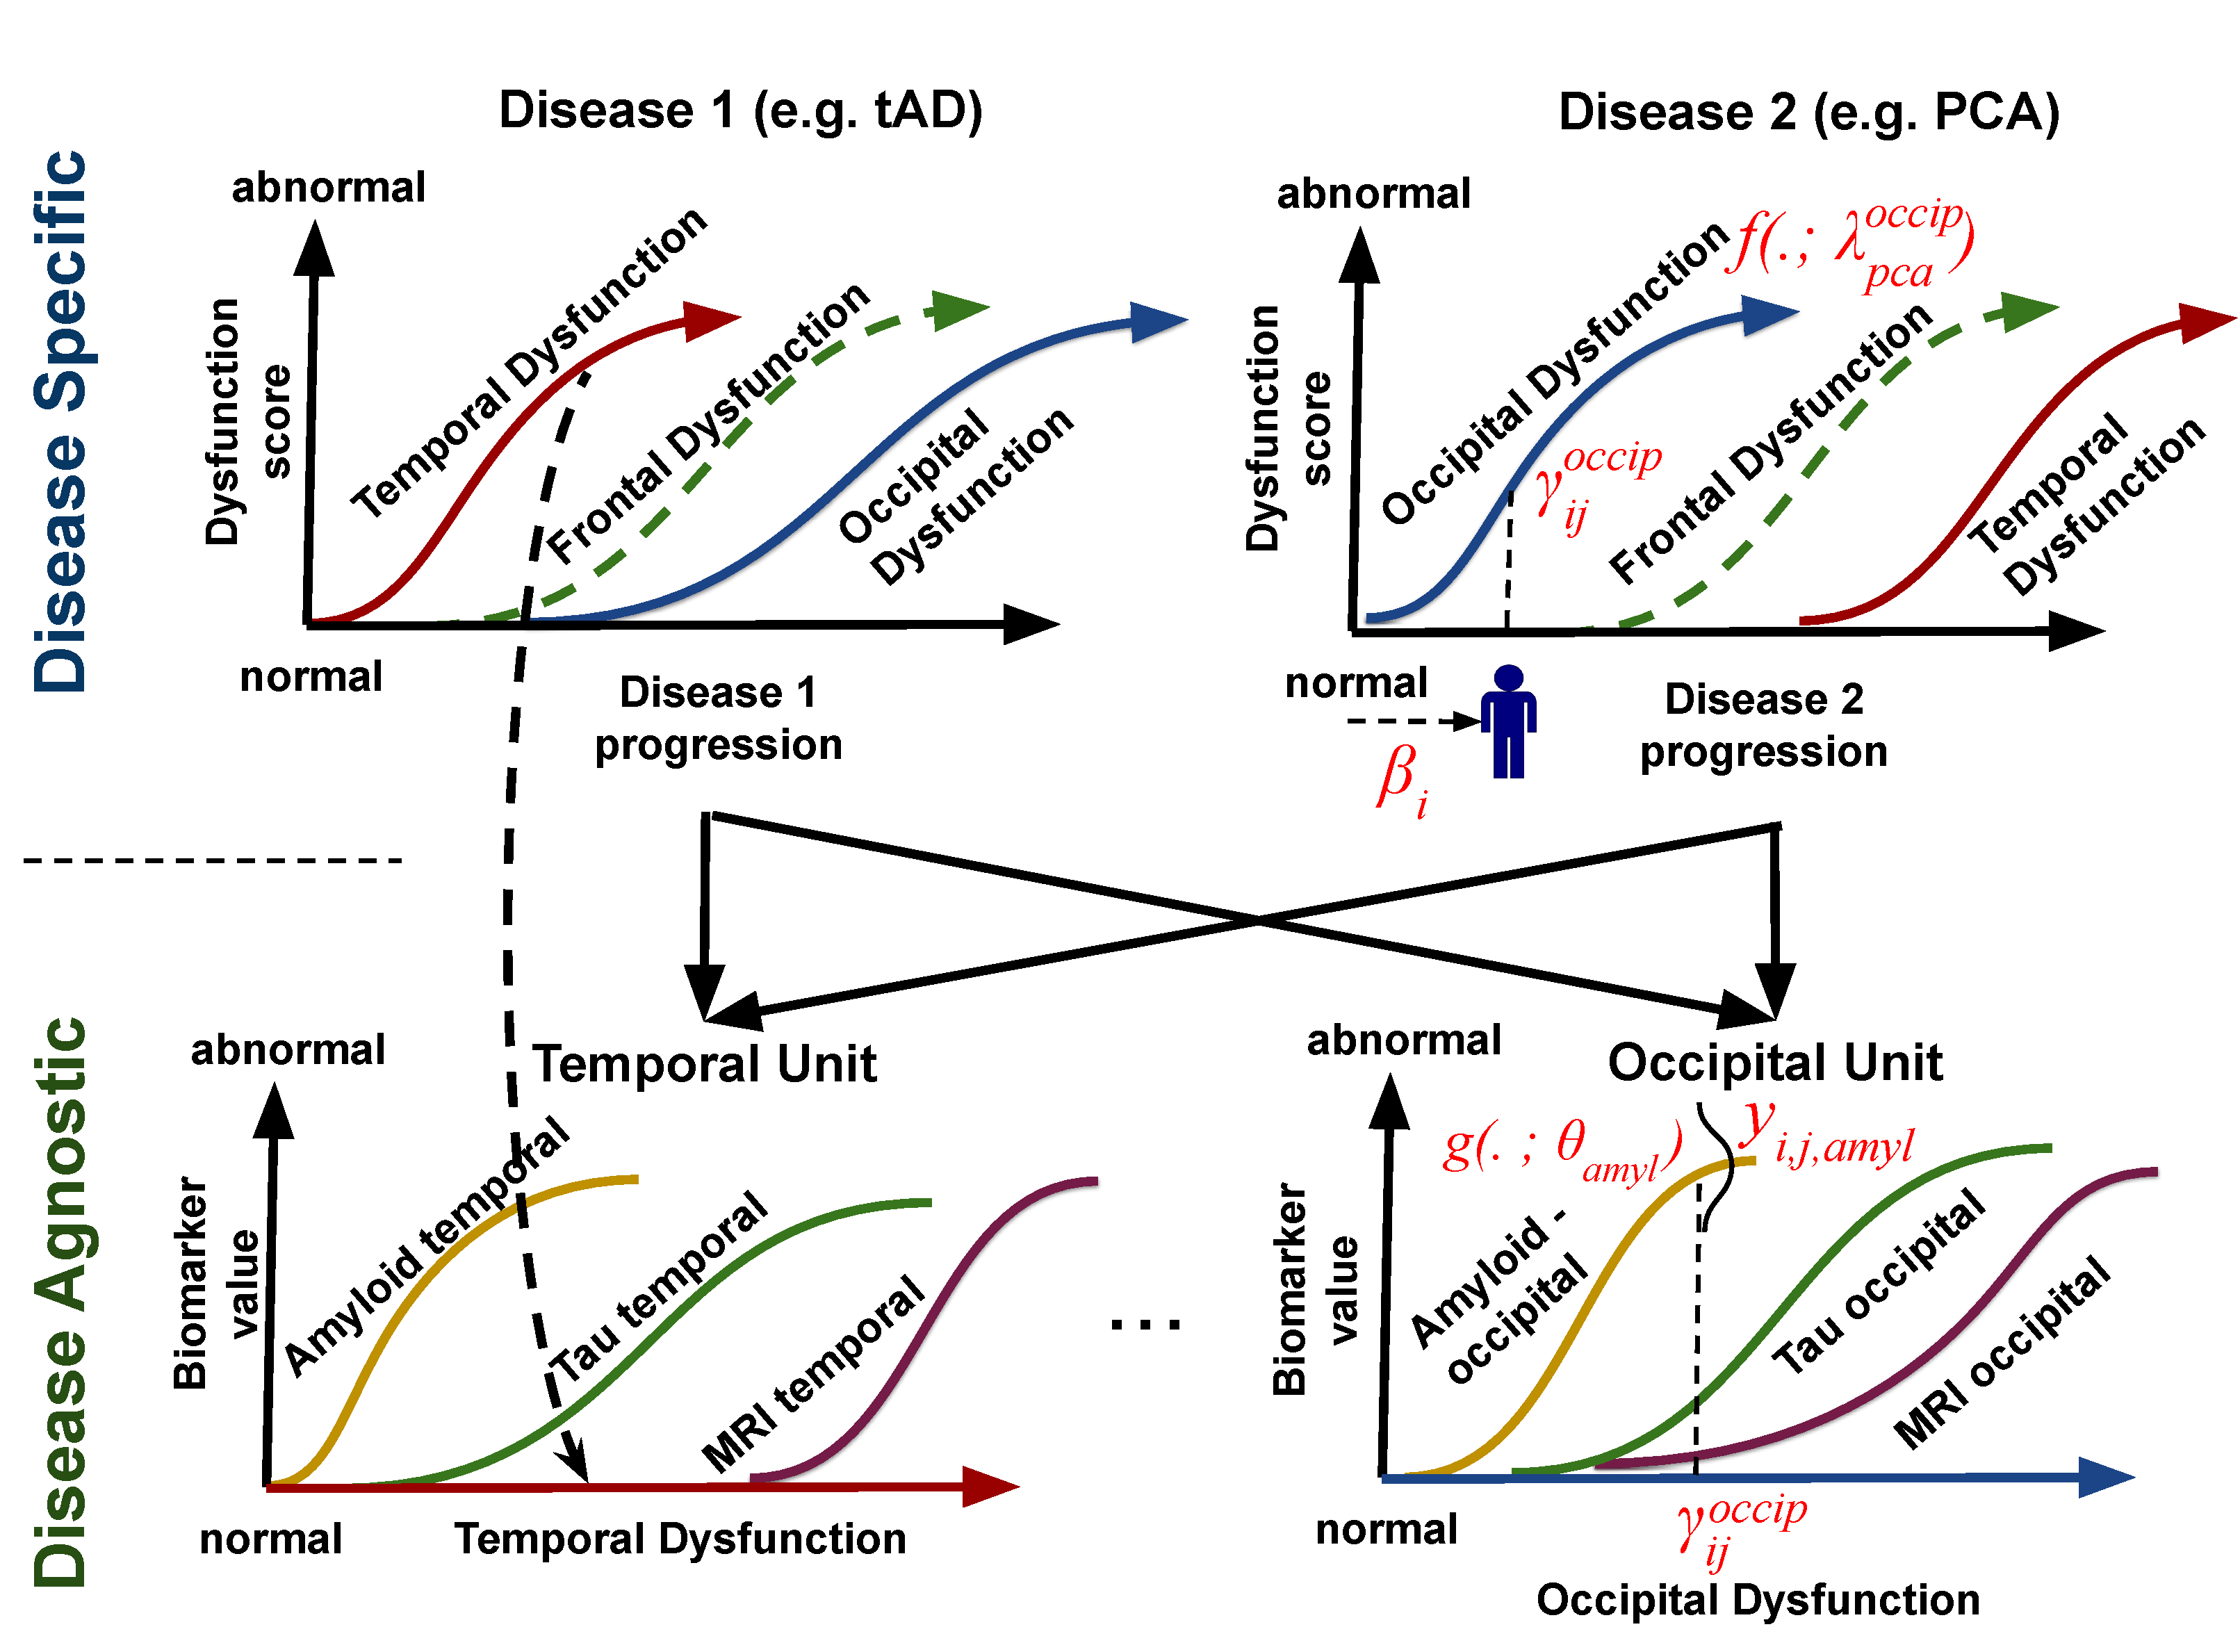
\includegraphics[width=\columnwidth]{../figures/disease_knowledge_transfer_symbols.pdf}
%  \caption{}
%  \label{fig:diagram}
\end{figure}



\section*{Results}


\begin{figure}[H]
\fnt{Synthetic experiment shows that the model can recover the underlying parameters}\\
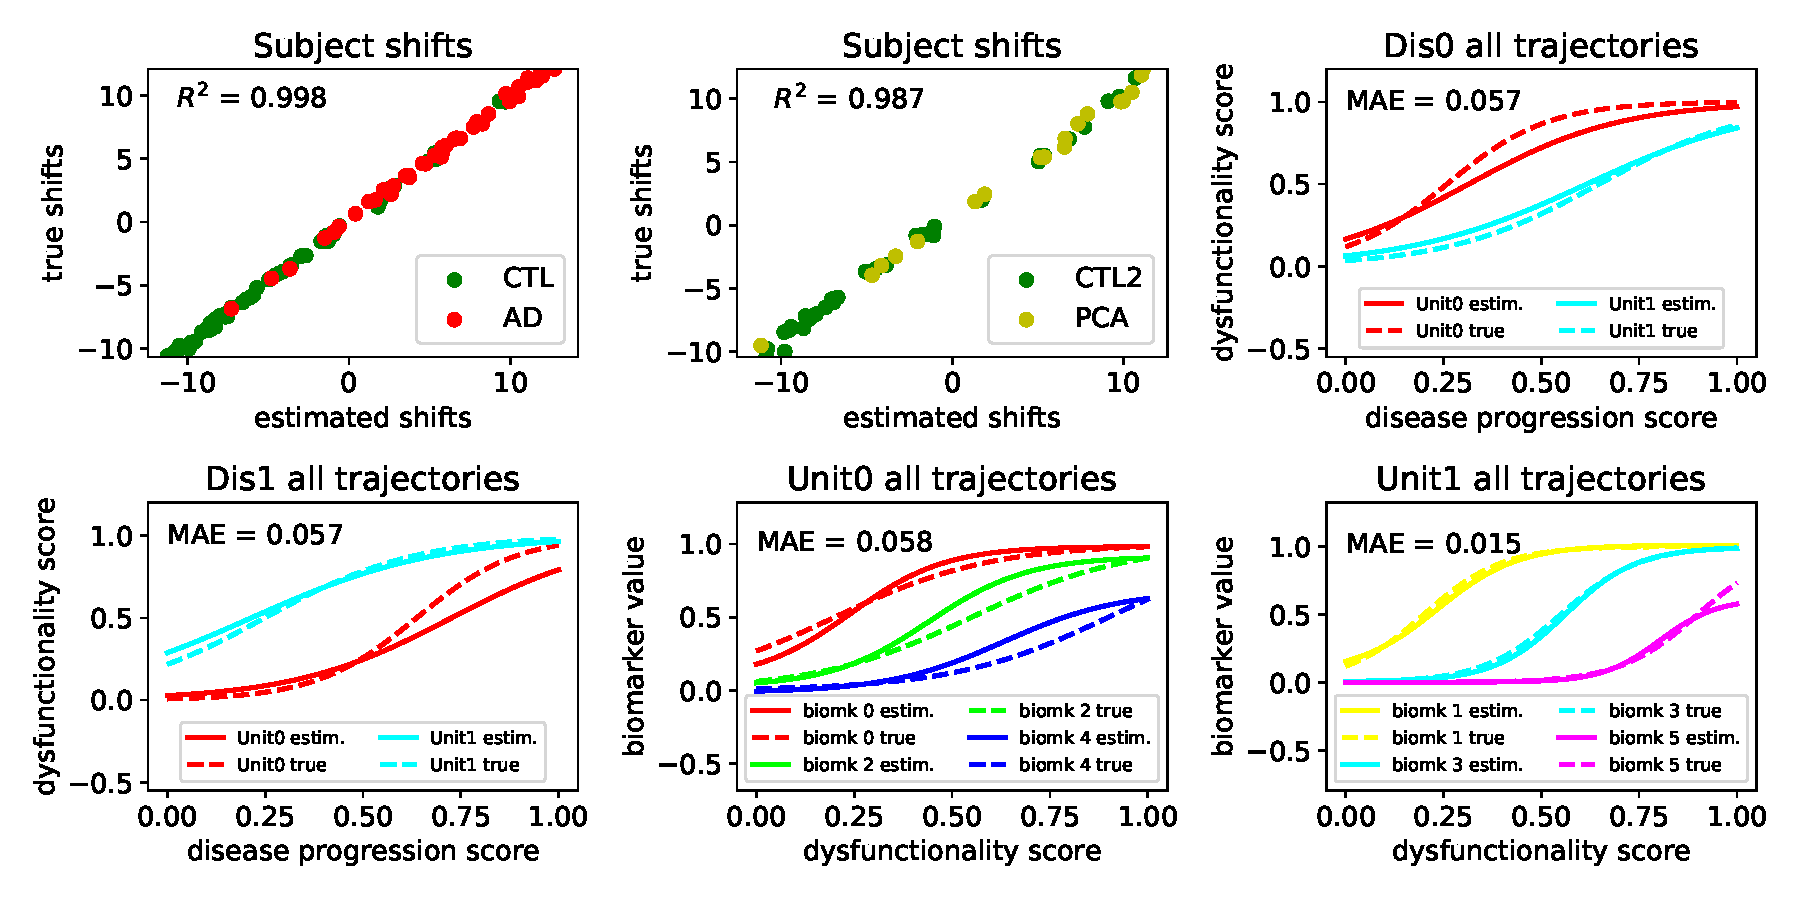
\includegraphics[width=0.4\textwidth]{../figures/compTrueParams105_synth1_JMD.pdf}
  \label{fig:dktSynthTrajCompTrue}
\end{figure}

\begin{figure}[H]
\centering
\fnt{Inferred trajectories for Posterior Cortical Atrophy}\\
 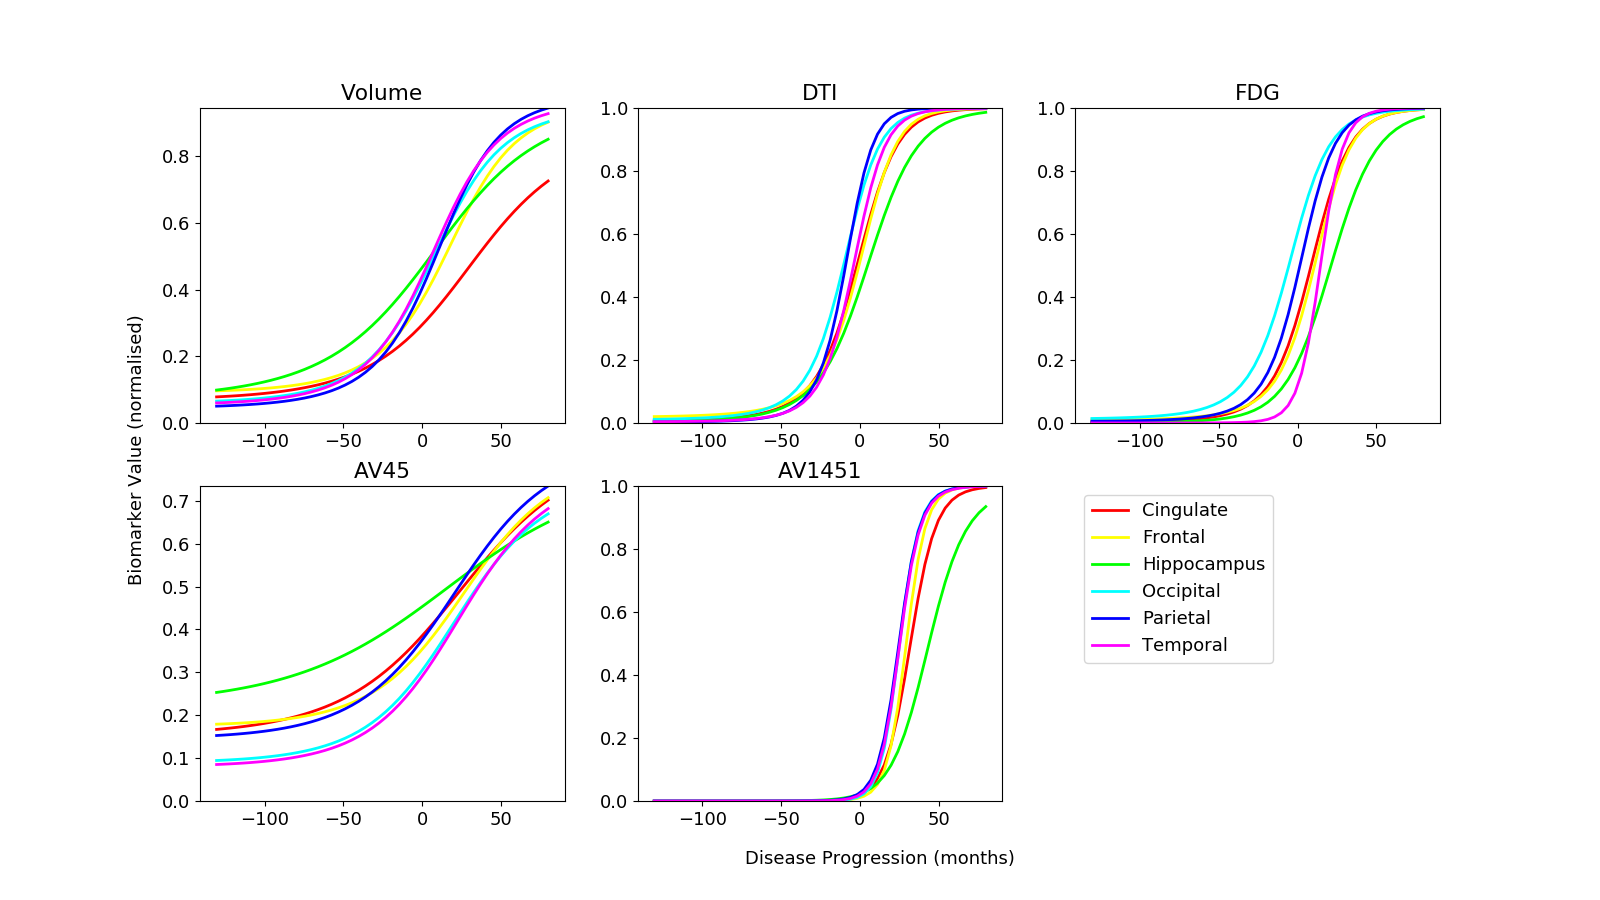
\includegraphics[width=0.4\textwidth, trim=0 20 0 0, clip]{../figures/trajDisSpaceOverlap_PCA_tad-drcTinyPen5_JMD.png}
%  \caption{Estimated trajectories for the PCA cohort. The only data that were available were the MRI volumetric data. The dynamics of the other biomarkers has been inferred by the model using data from typical AD, and taking into account the different spatial distribution of pathology in PCA vs tAD. }
%  \label{fig:PCAtrajByModality}
\end{figure}


\begin{table}[H]
\centering
\fnt{Our model has favourable performance compared to other models}\\
\vspace{1em}
\fontsize{27}{30}\selectfont
\begin{tabular}{c | c c c c c c}
\textbf{Model} & \textbf{Cingulate} & \textbf{Frontal} & \textbf{Hippocam.} & \textbf{Occipital} & \textbf{Parietal} & \textbf{Temporal}\\
& \multicolumn{6}{c}{\textbf{TADPOLE: Hippocampal subgroup to Cortical subgroup}}\\
DKT (ours) &      0.56 $\pm$ 0.23 &    \textbf{0.35 $\pm$ 0.17} &        \textbf{0.58 $\pm$ 0.14} &     -0.10 $\pm$ 0.29 &     \textbf{0.71 $\pm$ 0.11} &     \textbf{0.34 $\pm$ 0.26} \\
Latent stage &      0.44 $\pm$ 0.25 &    0.34 $\pm$ 0.21 &       0.34 $\pm$ 0.24* &     \textbf{-0.07 $\pm$ 0.22} &     0.64 $\pm$ 0.16 &    0.08 $\pm$ 0.24* \\
Multivariate &      \textbf{0.60 $\pm$ 0.18} &   0.11 $\pm$ 0.22* &       0.12 $\pm$ 0.29* &     -0.22 $\pm$ 0.22 &   -0.44 $\pm$ 0.14* &   -0.32 $\pm$ 0.29* \\
Spline &    -0.24 $\pm$ 0.25* &  -0.06 $\pm$ 0.27* &        0.58 $\pm$ 0.17 &     -0.16 $\pm$ 0.27 &    0.23 $\pm$ 0.25* &    0.10 $\pm$ 0.25* \\
Linear &    -0.24 $\pm$ 0.25* &   0.20 $\pm$ 0.25* &        0.58 $\pm$ 0.17 &     -0.16 $\pm$ 0.27 &    0.23 $\pm$ 0.25* &    0.13 $\pm$ 0.23* \\
& \multicolumn{6}{c}{\textbf{typical Alzheimer's to Posterior Cortical Atrophy}}\\
DKT (ours) &    0.77 $\pm$ 0.11 &    0.39 $\pm$ 0.26 &      0.75 $\pm$ 0.09 &    0.60 $\pm$ 0.14 &    \textbf{0.55 $\pm$ 0.24} &    \textbf{0.35 $\pm$ 0.22} \\
Latent stage &    \textbf{0.80 $\pm$ 0.09} &    \textbf{0.53 $\pm$ 0.17} &      \textbf{0.80 $\pm$ 0.12} &    0.56 $\pm$ 0.18 &    0.50 $\pm$ 0.21 &    0.32 $\pm$ 0.24 \\
Multivariate &   0.73 $\pm$ 0.09 &   0.45 $\pm$ 0.22  &    0.71 $\pm$ 0.08 & -0.28 $\pm$ 0.21* &  0.53 $\pm$ 0.22  &  0.25 $\pm$ 0.23* \\
Spline &   0.52 $\pm$ 0.20* &  -0.03 $\pm$ 0.35* &     0.66 $\pm$ 0.11* &   0.09 $\pm$ 0.25* &    0.53 $\pm$ 0.20 &   0.30 $\pm$ 0.21* \\
Linear &   0.52 $\pm$ 0.20* &    0.34 $\pm$ 0.27 &     0.66 $\pm$ 0.11* &    \textbf{0.64 $\pm$ 0.17} &    0.54 $\pm$ 0.22 &   0.30 $\pm$ 0.21* \\
\end{tabular}
\vspace{0.5em}
% \caption[Performance evaluation of DKT and other models]{Performance evaluation of DKT and four other statistical models of decreasing complexity. }
% \end{footnotesize}
\label{sec:dktPerfMetrics}
\end{table}


\section*{Conclusion}






\end{multicols}
\hrule


}


\begin{multicols}{2}
 							%Use 3-column layout
\raggedcolumns	

\subsection*{References}

\large{
\begin{tabular}{l p{0.5cm} l}
 1. Fontejin et al., Neuroimg., 2012 & & 2. Young et al., Nat. Comms., 2018\\
 3. Villemagne et al., Lancet Neurol., 2013 & & 4. Marinescu et al., IPMI, 2017\\
\end{tabular}

\columnbreak

\subsection*{Weblinks}
\begin{itemize}
\item UCL Progression of Neurodegenerative Disease (POND): cmic.cs.ucl.ac.uk/pond/
\item UCL Centre for Medical Image Computing: www.ucl.ac.uk/cmic/
\end{itemize}
}


\vspace{1em}
% \hspace{2em}

\includegraphics[height=4.0cm]{epsrc_logo.jpg}
\hspace{0.5em}

\includegraphics[height=4.0cm]{pondLogo.png} 
\hspace{0.5em}

\includegraphics[height=4cm]{cdt_logo.png} 
\hspace{0.5em}

\includegraphics[height=4cm]{aruk_logo} 


\end{multicols}


\end{document}
